\documentclass[12pt]{article}
\usepackage{amsthm}
\usepackage{amsmath}
\usepackage{amssymb}
\usepackage{natbib}
\usepackage{geometry}
\usepackage{tikz}
\usepackage{algorithm}
\usepackage{algpseudocode}
\usepackage{hyperref}

\usetikzlibrary{shapes.geometric, arrows.meta, positioning}
\geometry{margin=1in}

\theoremstyle{definition}
\newtheorem{definition}{Definition}[section]

\theoremstyle{plain}
\newtheorem{theorem}{Theorem}[section]
\newtheorem{proposition}{Proposition}[section]
\newtheorem{lemma}{Lemma}[section]

\title{The Flaws of Others}
\author{
    Juan B. Gutiérrez\footnote{\href{mailto:juan.gutierrez3@utsa.edu}{juan.gutierrez3@utsa.edu} Department of Mathematics, University of Texas at San Antonio.}
    % 
    %nd 
    %
}
\date{}

\begin{document}

\maketitle

\begin{abstract}
% To be written at the end.
\end{abstract}


%===============================================
\section{Introduction}
%===============================================

Large Language Models (LLMs) are advanced artificial intelligence systems trained on vast amounts of text data to generate human-like language. These models utilize deep learning techniques to understand and produce text based on the patterns and structures found in their training data \citep{vaswani2017attention, brown2020language}. LLMs have demonstrated impressive capabilities in various natural language processing tasks, including text generation, translation, and question-answering.

Despite their remarkable performance, LLMs are prone to generating false or misleading statements, a phenomenon often referred to as "hallucinations" \citep{ji2022survey}. Hallucinations in LLMs can manifest as factual inconsistencies, logical contradictions, or entirely fabricated content that appears plausible \citep{maynez2020faithfulness}. This issue is exacerbated by the lack of a verification mechanism within the models themselves \citep{bender2021dangers, weidinger2021ethical}.

Several factors contribute to the occurrence of hallucinations, including biases in training data, limitations in knowledge representation, and the models' tendency to prioritize fluency over factual accuracy \citep{lin2022truthfulqa}. The prevalence and impact of hallucinations are significant, with quantitative evaluations revealing that they occur in up to 30\% of generated responses, substantially affecting the trustworthiness of these models \citep{ji2022survey, lin2022truthfulqa}. Moreover, studies have shown that LLMs can generate false information even when explicitly prompted to be truthful \citep{evans2021truthful}, underscoring the challenge of aligning model outputs with factual correctness.

To address this problem, researchers have developed various mitigation strategies. These include techniques such as retrieval-augmented generation \citep{lewis2020retrieval}, which aims to ground model responses in external knowledge sources, and self-consistency checks \citep{wang2023self}, which attempt to improve the internal coherence of model outputs. Despite these efforts, hallucinations remain a significant challenge in the development of reliable AI systems.

The persistence of this issue highlights the need for ongoing research and development of robust verification methods. As LLMs continue to evolve and find applications in diverse fields, ensuring their factual accuracy and reliability becomes increasingly crucial. This challenge sits at the intersection of natural language processing, knowledge representation, and AI ethics, requiring interdisciplinary approaches to develop comprehensive solutions. 

%===============================================
\subsection{Invalidation vs. Hallucination}
%===============================================
While hallucinations in LLMs have been extensively studied, this paper introduces a novel concept called ``invalidation," which represents a distinct and potentially more insidious form of false information generation. Invalidation differs from hallucination in several key aspects:

1. Nature of Falsehood: Hallucinations are unintentional factual inaccuracies or fabrications, whereas invalidation involves the active negation or disputation of established truths.

2. Presentation of Information: Hallucinations typically result in plausible but incorrect information. In contrast, invalidation often presents alternative facts or misleading evidence that directly contradicts known truths.

3. Impact on Knowledge Systems: Hallucinations may lead to isolated errors, but invalidation has the potential to undermine entire systems of knowledge by creating doubt and confusion about verified facts.

4. Underlying Mechanisms: Hallucinations stem from the model's probabilistic nature and limitations in training data. Invalidation, while not intentional, appears more deliberate due to the emergent behavior of the model and the influence of biased or misleading training data.

For example, a hallucination might involve an LLM incorrectly stating the year of a historical event. Invalidation, on the other hand, might manifest as the LLM generating content that denies well-established scientific facts, such as climate change, by presenting fabricated data or misinterpreting genuine information.

This distinction between hallucination and invalidation is crucial for several reasons:

1. It allows for more targeted mitigation strategies, as the approaches needed to address invalidation may differ from those used for hallucinations.

2. It highlights a potentially more dangerous form of misinformation that could have far-reaching consequences in fields such as science, politics, and public health.

3. It emphasizes the need for more sophisticated verification mechanisms that can not only check factual accuracy but also detect attempts to undermine established knowledge.

To comprehensively understand and address these phenomena, we propose an epistemological framework that categorizes false information generated by LLMs into two distinct types: hallucination and invalidation. This framework helps delineate the nature, causes, and implications of each type, thus guiding the development of targeted mitigation strategies.

%===============================================
\subsection{Epistemological Framework for False Information}
%===============================================

1. Hallucination: Characterized by unintentional factual inaccuracies and fabrications due to the probabilistic text generation process. Mitigation strategies include improving training data quality, enhancing model architectures to prioritize factual accuracy, and incorporating real-time fact-checking mechanisms \citep{lewis2020retrieval, wang2023self}. For example, an LLM might generate a fabricated historical event due to the patterns it learned from the training data.

2. Invalidation: Defined by statements that negate or contradict established facts through misleading narratives or false evidence. Addressing invalidation requires methods to cross-verify generated content with credible sources and detect contradictions with known truths. Techniques like retrieval-augmented generation and consistency checks can be effective \citep{evans2021truthful}. For instance, generating false data to deny climate change exemplifies invalidation.

By distinguishing between these two types of false information, this framework not only aids in understanding the underlying mechanisms but also informs the development of more precise and effective countermeasures. Such an approach is critical in enhancing the reliability and trustworthiness of AI-driven language models, particularly as they become increasingly integrated into various domains of society. This framework also highlights important considerations in the broader context of AI ethics and the ongoing development of LLMs.

To address the problem of invalidation, some approaches suggest using multiple LLMs to cross-verify information \citep{li2021multiview}. By generating a consensus among different models, it is possible to reduce the likelihood of false statements. This method leverages the diverse training backgrounds and potential error distributions of multiple models, enhancing the overall accuracy and reliability of the generated content.

%===============================================
\subsection{Invalidation in Human Discourse and Its Universal Implications}
%===============================================

Invalidation, as observed in LLMs, is not an isolated phenomenon unique to artificial intelligence. Rather, it mirrors a well-documented pattern in human discourse, suggesting a potentially universal cognitive process that transcends the boundaries between artificial and human intelligence.

In social interactions, humans frequently encounter and sometimes generate statements that contradict observable evidence or present fabricated narratives as facts. This phenomenon manifests in various forms, from the denial of scientifically proven phenomena to the propagation of conspiracy theories. The parallel between human and LLM behavior in this regard is striking and warrants deeper exploration.

Sociological perspectives offer valuable insights into this phenomenon. \citet{goffman1959presentation} illuminates how individuals shape and present narratives that may invalidate certain states of the world, a process strikingly similar to the way LLMs construct alternative realities. \citet{festinger1957cognitive} theory of cognitive dissonance explains how people manage conflicting information and beliefs, often leading to the dismissal of evidence that contradicts their views - a process that may be analogous to how LLMs prioritize internal consistency over factual accuracy. \citet{cohen2001states} work on states of denial further illustrates how groups may collectively reject realities such as human rights violations, mirroring the way LLMs can generate content that negates established facts.

The field of media studies and communication theory provides additional parallels. \citet{mcluhan1964understanding} insights into how different media forms influence the dissemination and acceptance of information, including falsehoods, can be extended to understand how the architecture of LLMs shapes their output. \citet{chomsky1988manufacturing} analysis of how mass media shapes public perception by filtering and framing information resonates with the way LLMs process and generate content based on their training data. \citet{gerbner1976cultivation} cultivation theory, examining how prolonged exposure to media content can alter perceptions of reality, offers a framework for understanding how repeated exposure to certain patterns in training data might lead LLMs to generate invalidating content.

Political science and propaganda studies further illuminate this phenomenon. \citet{arendt1951origins} discussions on the use of propaganda to manipulate public perception find echoes in the way LLMs can generate misleading narratives. \citet{ellul1965propaganda} detailed analysis of how propaganda shapes beliefs and attitudes, leading to the invalidation of certain truths, provides a lens through which we can understand the potential societal impact of LLM-generated invalidations.

From a cognitive science perspective, \citet{kahneman1974judgment} work on heuristics and biases offers a framework for understanding why both humans and LLMs may accept and generate false narratives. \citet{pinker2002blank} exploration of how ideological beliefs can lead to the rejection of scientific evidence provides insight into the mechanisms behind invalidation in both human and artificial systems.

The striking parallels between invalidation in human discourse and in LLMs point to a potentially universal phenomenon rooted in the fundamental processes of information processing and knowledge representation. This similarity suggests that invalidation may not be merely a flaw in AI systems, but rather a manifestation of broader cognitive patterns that emerge in any sufficiently complex information processing system, whether biological or artificial.

Understanding invalidation as a universal phenomenon has profound implications for AI development and our broader understanding of cognition. It suggests that addressing invalidation in LLMs may require insights from diverse fields such as sociology, psychology, and cognitive science, in addition to computer science. Moreover, studying how LLMs produce invalidations may provide new perspectives on human cognitive processes, potentially offering insights into phenomena like confirmation bias, belief perseverance, and the spread of misinformation in human societies.

%===============================================
\subsection{Goal}
%===============================================
In this paper, we... [state the focus and contribution of the manuscript... to be done last based on all pieces that can be harmonized]

%===============================================
\section{Methods}
%===============================================
\subsection{Formalization of Invalidation}
%===============================================

To systematically study the phenomenon of invalidation, we propose a formal model that quantifies how invalidations propagate within a discursive network. This model considers actors as nodes in a network, with edges representing the exchange of statements. The goal is to understand how actors influence each other and how invalidations spread, eventually reaching an equilibrium state. The subsequent section will detail the methods used to develop and analyze this model, providing a quantitative framework for studying invalidation in both human and artificial contexts.

%===============================================
\subsection{Basic Invalidation Propagation}
%===============================================

\begin{definition}\label{def:actors_statements}
\textbf{Actors and Statements.} Let $A = \{a_1, a_2, \ldots, a_n\}$ be the set of actors in the discursive network, and let $S = \{s_1, s_2, \ldots, s_m\}$ be the set of all possible statements in the network, where each statement $s_i$ can be either true or false.
\end{definition}

\begin{proposition}\label{prop:beliefs_goals}
Each actor $a_i$ holds a set of beliefs, represented by $B_i \subseteq S$. A belief is a statement that the actor considers true. The goal function $G_i$, $G_i: A \to 2^S$, the power set of $S$, represents the set of statements $a_i$ aims to convince $a_j$ to believe. This includes every combination of elements that can be formed from $S$, ranging from the empty set to the full set $S$ itself. 
\end{proposition}

\begin{proposition}\label{prop:communication_invalidation}
Communication between actors involves the exchange of statements. A communication from actor $a_i$ to actor $a_j$ is represented as $C_{ij} = \{s_k \mid s_k \in B_i \}$, where $s_k$ is a statement that $a_i$ believes and wants $a_j$ to accept. Invalidation occurs when an actor presents a statement that directly contradicts another statement or fabricates evidence to support a false proposition. Formally, $I_{ij}(s_k, s_l)$ denotes that actor $a_i$ invalidates statement $s_k$ held by $a_j$ by presenting $s_l$.
\end{proposition}

\begin{proposition}\label{prop:persuasion_update}
The persuasion function $P_{ij}(s_k)$ represents the likelihood that actor $a_j$ will adopt statement $s_k$ after communication from $a_i$. This can be modeled using probabilities or influence weights. The update rule $U_j(B_j, C_{ij}, I_{ij})$ determines how the belief set $B_j$ of actor $a_j$ is updated after receiving communication $C_{ij}$ from actor $a_i$ and experiencing invalidation $I_{ij}$.
\end{proposition}

\begin{proposition}\label{prop:formal_model}
Let $N = (A, S, B, G, C, I, P, U)$ be the formal model of the discursive network, where $A$ is the set of actors, $S$ is the set of statements, $B = \{B_1, B_2, \ldots, B_n\}$ is the set of belief sets for each actor, $G = \{G_1, G_2, \ldots, G_n\}$ is the set of goal functions for each actor, $C = \{C_{ij} \mid i, j \in \{1, 2, \ldots, n\}\}$ is the set of communications between actors, $I = \{I_{ij} \mid i, j \in \{1, 2, \ldots, n\}\}$ is the set of invalidations between actors, $P = \{P_{ij} \mid i, j \in \{1, 2, \ldots, n\}\}$ is the set of persuasion functions, and $U = \{U_j \mid j \in \{1, 2, \ldots, n\}\}$ is the set of update rules.
\end{proposition}

\textbf{Example.} Consider a simple scenario with three actors $A = \{a_1, a_2, a_3\}$ and two statements $S = \{s_1, s_2\}$. Actor $a_1$ believes $s_1$ ($B_1 = \{s_1\}$) and wants $a_2$ and $a_3$ to also believe $s_1$ ($G_1(a_2) = G_1(a_3) = \{s_1\}$). Actor $a_2$ believes $s_2$ ($B_2 = \{s_2\}$) and wants $a_1$ and $a_3$ to believe $s_2$ ($G_2(a_1) = G_2(a_3) = \{s_2\}$). Actor $a_3$ is initially neutral ($B_3 = \emptyset$). Actor $a_1$ communicates $C_{12} = \{s_1\}$ to $a_2$, who invalidates $s_1$ by presenting $I_{21}(s_1, s_2)$. Actor $a_3$, observing this interaction, updates their belief set based on the persuasion functions and update rules. This framework models the propagation of invalidation within a discursive network, capturing the dynamics of belief, communication, and influence. By formalizing these interactions, we can analyze and predict how invalidation affects the acceptance and rejection of statements among actors in the network.

\begin{proposition}\label{prop:basic_model_formulation}
\textbf{Basic Model Formulation.} To describe the state of asymptotic equilibrium of the system mathematically, we need to analyze the transition probabilities between the states $s_1$ and $s_2$. This can be modeled using a Markov chain with two states.
\end{proposition}

Define the states as follows: $S_1$: The state where an actor believes $s_1$. $S_2$: The state where an actor believes $s_2$. The transition probabilities are: $p_{12}$: Probability that an actor transitions from $S_1$ to $S_2$, and $p_{21}$: Probability that an actor transitions from $S_2$ to $S_1$. Let $P(t)$ represent the state vector at time $t$, where: $P_1(t)$: Proportion of actors in state $S_1$ at time $t$ and $P_2(t)$: Proportion of actors in state $S_2$ at time $t$. 

The transition matrix $T$ is given by:
\begin{equation}\label{eq:transition_matrix}
T = \begin{pmatrix}
1 - p_{12} & p_{12} \\
p_{21} & 1 - p_{21}
\end{pmatrix}
\end{equation}

The state vector $P(t)$ evolves according to:
\begin{equation}\label{eq:state_vector_evolution}
P(t+1) = T \cdot P(t) 
\end{equation}


\begin{theorem}\label{thm:basic_invalidation_propagation}
\textbf{Basic Invalidation Propagation.} The state of equilibrium of  the system described by Equation \ref{eq:state_vector_evolution} is a stable fixed point given by:
\[
P = \begin{pmatrix}
\frac{p_{21}}{p_{12} + p_{21}} \\
\frac{p_{12}}{p_{12} + p_{21}}
\end{pmatrix}
\]
\end{theorem}

\textbf{Proof.} The system reaches equilibrium when $P(t+1) = P(t) = P$, where $P$ is the equilibrium state vector. At equilibrium, the proportions of actors holding each belief remain constant. We need to solve the equation:
\begin{equation}\label{eq:equilibrium_condition}
P  =  T \cdot P.
\end{equation}
%
This can be written as a system of linear equations:
%
\begin{equation}\label{eq:linear_system}
    \begin{pmatrix}
        P_1 \\ 
        P_2
    \end{pmatrix}
    = 
    \begin{pmatrix}
        1 - p_{12} & p_{21} \\
        p_{12} & 1 - p_{21}
    \end{pmatrix}
    \begin{pmatrix}
        P_1 \\ 
        P_2
    \end{pmatrix},
\end{equation}
%
or in agebraic form
%
\begin{align}
    P_1 & = (1 - p_{12}) P_1  +  p_{21} P_2 \label{eq:equilibrium_eq1}, \\
    P_2 & = p_{12} P_1  +  (1 - p_{21}) P_2 \label{eq:equilibrium_eq2}.
\end{align}
%
Rearraging, we obtain 
%
\begin{align}
    P_1 & = P_1 - p_{12} P_1  + p_{21} P_2, \\
    P_2 & = p_{12} P_1  + P_2 - p_{21} P_2.  
\end{align}
%
Ssimplifying, 
%
\begin{align}
    - P_1 p_{12} + P_2 p_{12} &= 0 \label{eq:equilibrium_simplify1} \\
    P_1 p_{12} & = P_2 p_{12}
\end{align}
%
Since $p_{12} \neq 0$:
%
\begin{equation}\label{eq:equilibrium_simplify2}
    P_1 = P_2 \cdot \frac{p_{21}}{p_{12}}
\end{equation}
%
From the normalization condition $P_1 + P_2 = 1$:
%
\begin{equation}\label{eq:normalization_condition}
P_2 \cdot \frac{p_{21}}{p_{12}} + P_2 = 1 
\end{equation}
%
from where 
%
\begin{equation}\label{eq:normalization_condition}
P_2 = \frac{p_{12}}{p_{12} + p_{21}}
\end{equation}
%
Substitute $P_2$ back into the equation for $P_1$:
\begin{align}\label{eq:equilibrium_proportion1}
    P_1 =& \frac{p_{21}}{p_{12}} \cdot P_2 \\ 
    P_1 =& \frac{p_{21}}{p_{12} + p_{21}}
\end{align}
%
Thus, the equilibrium state vector is:
%
\begin{equation}\label{eq:equilibrium_proportions}
P = \begin{pmatrix}
P_1 \\
P_2
\end{pmatrix}
=
\begin{pmatrix}
\frac{p_{21}}{p_{12} + p_{21}} \\
\frac{p_{12}}{p_{12} + p_{21}}
\end{pmatrix}.
\end{equation}
%

Since system \ref{eq:state_vector_evolution} is linear, its stability can be assessed by determining the values of the roots of the characteristic polynomial resulting from assessing $\det(T-\lambda I) = 0$. The characteristic polynomial is 
%
\[
    {\lambda}^{2} + (p_{12} + p_{21} - 2) \, \lambda + 1 - p_{12}-p_{21}  = 0,
\]
%
resulting in the roots $\{1, 1 - p_{12}-p_{21}\}$. The stability of the first root is undecidable, but the secodn root is clearly less than one, which is the necessary and sufficient condition for stability fo discrete dynamical systems. Thus, the fixed point is stable. This completes the proof. \(\square\)

\textbf{Interpretation:} The proportion of actors holding belief $s_1$ is $P_1$ and the proportion of actors holding belief $s_2$ is $P_2$. When $p_{12} > p_{21}$, i.e., when the probability of transitioning from $s_1$ to $s_2$ is higher than the probability of transitioning from $s_2$ to $s_1$, more actors will shift their belief from $s_1$ to $s_2$ than from $s_2$ to $s_1$ over time.


\textbf{$P_1$ (Proportion of actors holding belief $s_1$)}: $P_1 = \frac{p_{21}}{p_{12} + p_{21}}$. Since $p_{12} > p_{21}$, $P_1$ will be less than 0.5. This means that fewer actors will hold belief $s_1$ at equilibrium compared to belief $s_2$.

\textbf{$P_2$ (Proportion of actors holding belief $s_2$)}: $P_2 = \frac{p_{12}}{p_{12} + p_{21}}$. Since $p_{12} > p_{21}$, $P_2$ will be greater than 0.5. This means that more actors will hold belief $s_2$ at equilibrium.

In summary, when $p_{12} > p_{21}$, the system will reach an equilibrium where the proportion of actors holding the belief $s_2$ is higher than the proportion of actors holding the belief $s_1$. This reflects the higher likelihood of actors transitioning from $s_1$ to $s_2$ compared to the reverse.


%===============================================
\subsection{Cross-Network Invalidation Detection Model}
%===============================================

We present an enhanced model of two interconnected discursive networks, each with the capacity to generate falsehoods internally and detect falsehoods in the other network. This refined model incorporates time-dependent parameters, accounts for network size effects, and allows for asymmetry between networks.

\begin{definition}\label{def:cross_networks}
\textbf{Dual Networks.} Let $N_1$ and $N_2$ be two discursive networks, with sets of actors $A_1 = \{a_{11}, a_{12}, ..., a_{1n_1}\}$ and $A_2 = \{a_{21}, a_{22}, ..., a_{2n_2}\}$ respectively, where $n_1$ and $n_2$ are the number of actors in each network. 
\end{definition}

\begin{proposition}\label{prop:network_state}
\textbf{Network State.} The state of each network $N_k$ at time $t$ is represented by $S_k(t) = (T_k(t), F_k(t))$, where $T_k(t)$ is the number of true statements and $F_k(t)$ is the number of false statements in network $N_k$ at time $t$.
\end{proposition}

\begin{proposition}\label{prop:falsehood_generation}
\textbf{Falsehood Generation.} Let $\lambda_k(t)$ be the rate at which new falsehoods are generated in network $N_k$ at time $t$, influenced by network dynamics and external factors. The number of new falsehoods generated in network $N_k$ at time $t$, denoted by $X_k(t)$, follows a Poisson distribution:

\begin{equation}
X_k(t) \sim \text{Poisson}(\lambda_k(t))
\end{equation}
\end{proposition}

\begin{proposition}\label{prop:cross_detection}
\textbf{Cross-Network Detection.} Let $d_{jk}(t)$ be the probability that a falsehood in network $N_k$ is detected by an actor in network $N_j$ at time $t$. The number of falsehoods detected and removed from network $N_k$ by network $N_j$ at time $t$, denoted by $Y_{jk}(t)$, follows a Binomial distribution:

\begin{equation}
Y_{jk}(t) \sim \text{Binomial}(F_k(t), d_{jk}(t))
\end{equation}
\end{proposition}

\begin{proposition}\label{prop:internal_dynamics}
\textbf{Internal Dynamics.} Let $p_k(t)$ be the probability that a true statement in network $N_k$ becomes false at time $t$, and $q_k(t)$ be the probability that a false statement in network $N_k$ is corrected to become true at time $t$. The number of true statements becoming false, $Z_k(t)$, and false statements becoming true, $W_k(t)$, in network $N_k$ at time $t$ follow Binomial distributions:

\begin{equation}
Z_k(t) \sim \text{Binomial}(T_k(t), p_k(t))
\end{equation}
\begin{equation}
W_k(t) \sim \text{Binomial}(F_k(t), q_k(t))
\end{equation}
\end{proposition}

The evolution of the network states can be described by the following stochastic difference equations:

\begin{equation}\label{eq:true_statements_evolution}
T_k(t+1) = T_k(t) - Z_k(t) + W_k(t)
\end{equation}

\begin{equation}\label{eq:false_statements_evolution}
F_k(t+1) = F_k(t) + X_k(t) + Z_k(t) - W_k(t) - Y_{jk}(t)
\end{equation}

\begin{theorem}\label{thm:expected_equilibrium}
\textbf{Expected Equilibrium State.} The expected equilibrium state of network $N_k$ is given by:

\begin{equation}
E[T_k^*] = \frac{q_k^* n_k}{p_k^* + q_k^*} - \frac{\lambda_k^* n_k}{d_{jk}^*(p_k^* + q_k^*)}
\end{equation}

\begin{equation}
E[F_k^*] = \frac{\lambda_k^* n_k}{d_{jk}^*}
\end{equation}

where $n_k = E[T_k^*] + E[F_k^*]$ is the expected total number of statements in network $N_k$ at equilibrium, and $\lambda_k^*, d_{jk}^*, p_k^*, q_k^*$ are the long-term average values of the respective time-dependent parameters.
\end{theorem}


\begin{proof}
    \textbf{Step 1: Equilibrium Conditions}
    
    At equilibrium, the expected changes in true and false statements should be zero:
    
    \begin{equation}\label{eq:equilibrium_true}
    E[Z_k] = E[W_k]
    \end{equation}
    
    \begin{equation}\label{eq:equilibrium_false}
    E[X_k] = E[Y_{jk}] + E[W_k] - E[Z_k]
    \end{equation}
    
    \textbf{Step 2: Expected Values and Distribution Justifications}
    
    Express the expected values for each random variable, with detailed justifications for the choice of distributions:
    
    \begin{align}
    E[X_k] &= \lambda_k^* \quad \text{(Poisson distribution mean)} \\
    E[Y_{jk}] &= F_k^* \cdot d_{jk}^* \quad \text{(Binomial distribution mean)} \\
    E[Z_k] &= T_k^* \cdot p_k^* \quad \text{(Binomial distribution mean)} \\
    E[W_k] &= F_k^* \cdot q_k^* \quad \text{(Binomial distribution mean)}
    \end{align}
    
    1. $E[X_k] = \lambda_k^*$ (Poisson distribution mean):
       - The Poisson distribution is used to model the number of events occurring in a fixed interval of time or space, given a known average rate. In this case, $X_k$ represents the number of new falsehoods generated in network $N_k$. The parameter $\lambda_k^*$ is the average rate of falsehood generation at equilibrium.
    
    2. $E[Y_{jk}] = F_k^* \cdot d_{jk}^*$ (Binomial distribution mean):
       - $Y_{jk}$ represents the number of falsehoods in network $N_k$ detected by network $N_j$. This follows a Binomial distribution because each false statement in $N_k$ has a fixed probability $d_{jk}^*$ of being detected by $N_j$.
    
    3. $E[Z_k] = T_k^* \cdot p_k^*$ (Binomial distribution mean):
       - $Z_k$ represents the number of true statements in network $N_k$ that become false. This also follows a Binomial distribution because each true statement has a fixed probability $p_k^*$ of becoming false.
    
    4. $E[W_k] = F_k^* \cdot q_k^*$ (Binomial distribution mean):
       - $W_k$ represents the number of false statements in network $N_k$ that are corrected to become true. This follows a Binomial distribution as well, with $F_k^*$ false statements each having a probability $q_k^*$ of being corrected.
    
    \textbf{Step 3: Substitute Expected Values}
    
    Substitute these into our equilibrium equations:
    
    \begin{equation}\label{eq:equilibrium_true_substituted}
    T_k^* \cdot p_k^* = F_k^* \cdot q_k^*
    \end{equation}
    
    \begin{equation}\label{eq:equilibrium_false_substituted}
    \lambda_k^* = F_k^* \cdot d_{jk}^* + F_k^* \cdot q_k^* - T_k^* \cdot p_k^*
    \end{equation}
    
    \textbf{Step 4: Solve for $F_k^*$ in terms of $T_k^*$}
    
    From Equation \ref{eq:equilibrium_true_substituted}:
    
    \begin{equation}\label{eq:Fk_in_terms_of_Tk}
    F_k^* = T_k^* \cdot \frac{p_k^*}{q_k^*}
    \end{equation}
    
    \textbf{Step 5: Total Statements}
    
    The total number of statements $n_k$ is the sum of true and false statements:
    
    \begin{align}
    n_k &= T_k^* + F_k^* \\
    &= T_k^* + T_k^* \cdot \frac{p_k^*}{q_k^*} \\
    &= T_k^* \cdot \left(1 + \frac{p_k^*}{q_k^*}\right) \\
    &= T_k^* \cdot \frac{p_k^* + q_k^*}{q_k^*}
    \end{align}
    
    \textbf{Step 6: Solve for $T_k^*$}
    
    Rearranging the last equation from Step 5:
    
    \begin{equation}\label{eq:Tk_star}
    T_k^* = n_k \cdot \frac{q_k^*}{p_k^* + q_k^*}
    \end{equation}
    
    \textbf{Step 7: Solve for $F_k^*$}
    
    Substitute Equation \ref{eq:Tk_star} into Equation \ref{eq:Fk_in_terms_of_Tk}:
    
    \begin{align}
    F_k^* &= T_k^* \cdot \frac{p_k^*}{q_k^*} \\
    &= n_k \cdot \frac{q_k^*}{p_k^* + q_k^*} \cdot \frac{p_k^*}{q_k^*} \\
    &= n_k \cdot \frac{p_k^*}{p_k^* + q_k^*}
    \end{align}
    
    \textbf{Step 8: Use Equilibrium False Equation}
    
    From Equation \ref{eq:equilibrium_false_substituted}, substitute the expressions for $F_k^*$ and $T_k^*$:
    
    \begin{align}
    \lambda_k^* &= F_k^* \cdot d_{jk}^* + F_k^* \cdot q_k^* - T_k^* \cdot p_k^* \\
    &= n_k \cdot \frac{p_k^*}{p_k^* + q_k^*} \cdot d_{jk}^* + n_k \cdot \frac{p_k^*}{p_k^* + q_k^*} \cdot q_k^* - n_k \cdot \frac{q_k^*}{p_k^* + q_k^*} \cdot p_k^*
    \end{align}
    
    Here, we clearly show the intermediate steps of substitution.
    
    \textbf{Step 9: Simplify}
    
    Combine terms and simplify, showing each algebraic step:
    
    \begin{align}
    \lambda_k^* &= n_k \cdot \frac{p_k^* d_{jk}^* + p_k^* q_k^* - q_k^* p_k^*}{p_k^* + q_k^*} \\
    &= n_k \cdot \frac{p_k^* (d_{jk}^* + q_k^* - q_k^*)}{p_k^* + q_k^*} \\
    &= n_k \cdot \frac{p_k^* d_{jk}^*}{p_k^* + q_k^*}
    \end{align}
    
    \textbf{Step 10: Explicit Derivation for $F_k^*$}
    
    Rearrange the last equation to solve for $F_k^*$:
    
    \begin{align}
    \lambda_k^* &= n_k \cdot \frac{p_k^* d_{jk}^*}{p_k^* + q_k^*} \\
    \Rightarrow F_k^* &= \frac{\lambda_k^* \cdot (p_k^* + q_k^*)}{d_{jk}^*}
    \end{align}
    
    \textbf{Step 11: Final $T_k^*$}
    
    Subtract $F_k^*$ from $n_k$ to get the final expression for $T_k^*$:
    
    \begin{align}
    T_k^* &= n_k - F_k^* \\
    &= n_k - \frac{\lambda_k^* \cdot (p_k^* + q_k^*)}{d_{jk}^*} \\
    &= n_k \cdot \left(1 - \frac{\lambda_k^*}{d_{jk}^*}\right) \\
    &= \frac{q_k^* \cdot n_k}{p_k^* + q_k^*} - \frac{\lambda_k^* \cdot n_k}{d_{jk}^* \cdot (p_k^* + q_k^*)}
    \end{align}
    
    This completes the proof, deriving the expressions for $E[T_k^*]$ and $E[F_k^*]$ as stated in the theorem. \(\square\)
\end{proof}
    

\textbf{Interpretation and Analysis:}

1. Falsehood Generation vs. Detection: The ratio $\frac{\lambda_k^*}{d_{jk}^*}$ represents the balance between falsehood generation and cross-network detection. A higher ratio leads to more false statements at equilibrium.

2. Network Size Effect: Larger networks (higher $n_k$) can sustain more true and false statements at equilibrium. The number of false statements is now proportional to network size, reflecting increased opportunities for falsehood generation in larger discourse spaces.

3. Internal Dynamics: The ratio $\frac{q_k^*}{p_k^* + q_k^*}$ represents the proportion of non-false statements that are true at equilibrium due to internal dynamics.

4. Cross-Network Efficiency: Higher detection probabilities $d_{jk}^*$ lead to fewer false statements, highlighting the importance of cross-network scrutiny.

5. Asymmetry: Differences in parameters between networks can lead to asymmetric equilibrium states, potentially modeling real-world scenarios where one network is more susceptible to falsehoods or more efficient at detection.

6. Time-Dependent Dynamics: The model now captures how falsehood generation, detection, and internal correction processes may vary over time, allowing for more realistic modeling of network behavior.

7. Stochastic Nature: The use of Poisson and Binomial distributions introduces inherent randomness, reflecting the unpredictable nature of falsehood generation and detection in real-world scenarios.



%===============================================
\section{Results}
%===============================================
\subsection{Numerical Simulations}
%===============================================

[TO DO: Read, digest, ensure it is correct.]

This section details the numerical simulations implemented to explore the dynamics of belief systems within a discursive network. The simulations leverage a Markov chain model with dynamically adjusted transition probabilities, reflecting the interaction frequencies and statement validity.  

To simulate the interaction counts \( N_{s2}(t) \) involving the false statement \( s2 \) over time, a Poisson distribution is employed. The Poisson distribution is ideally suited for this purpose due to several key characteristics: (i) \textbf{Event independence:} The distribution assumes that each interaction is an independent event, a reasonable approximation given the diverse sources and triggers of discussions in a large network, (ii) \textbf{fixed average rate:} It is characterized by its rate parameter \( \lambda \), which simplifies modeling interactions that occur at a consistent average rate over time, (iii) \textbf{simplicity and mathematical tractability:} The Poisson distribution provides a straightforward formulation for calculating probabilities of occurrence for various numbers of interactions, facilitating the integration into stochastic models like Markov chains, and (iv)\textbf{flexibility in modeling sparse data:} It effectively handles data scenarios where interactions are rare or occur in bursts, typical of communication patterns in social networks.

The Python programming language was used to implement the simulation, employing the NumPy library for handling numerical operations and Matplotlib for visualizing the evolution of belief states over time. Initial states and parameters were set based on theoretical assumptions to reflect realistic interaction dynamics.

The simulation runs over a predefined number of time steps, updating the belief states according to the transition matrix \( T(t) \). The stability and convergence of the model are analyzed by observing changes in the proportions of belief states across the simulation period, providing insights into the long-term behavior of the network under varying interaction patterns.

\begin{figure}[h]
    \centering
    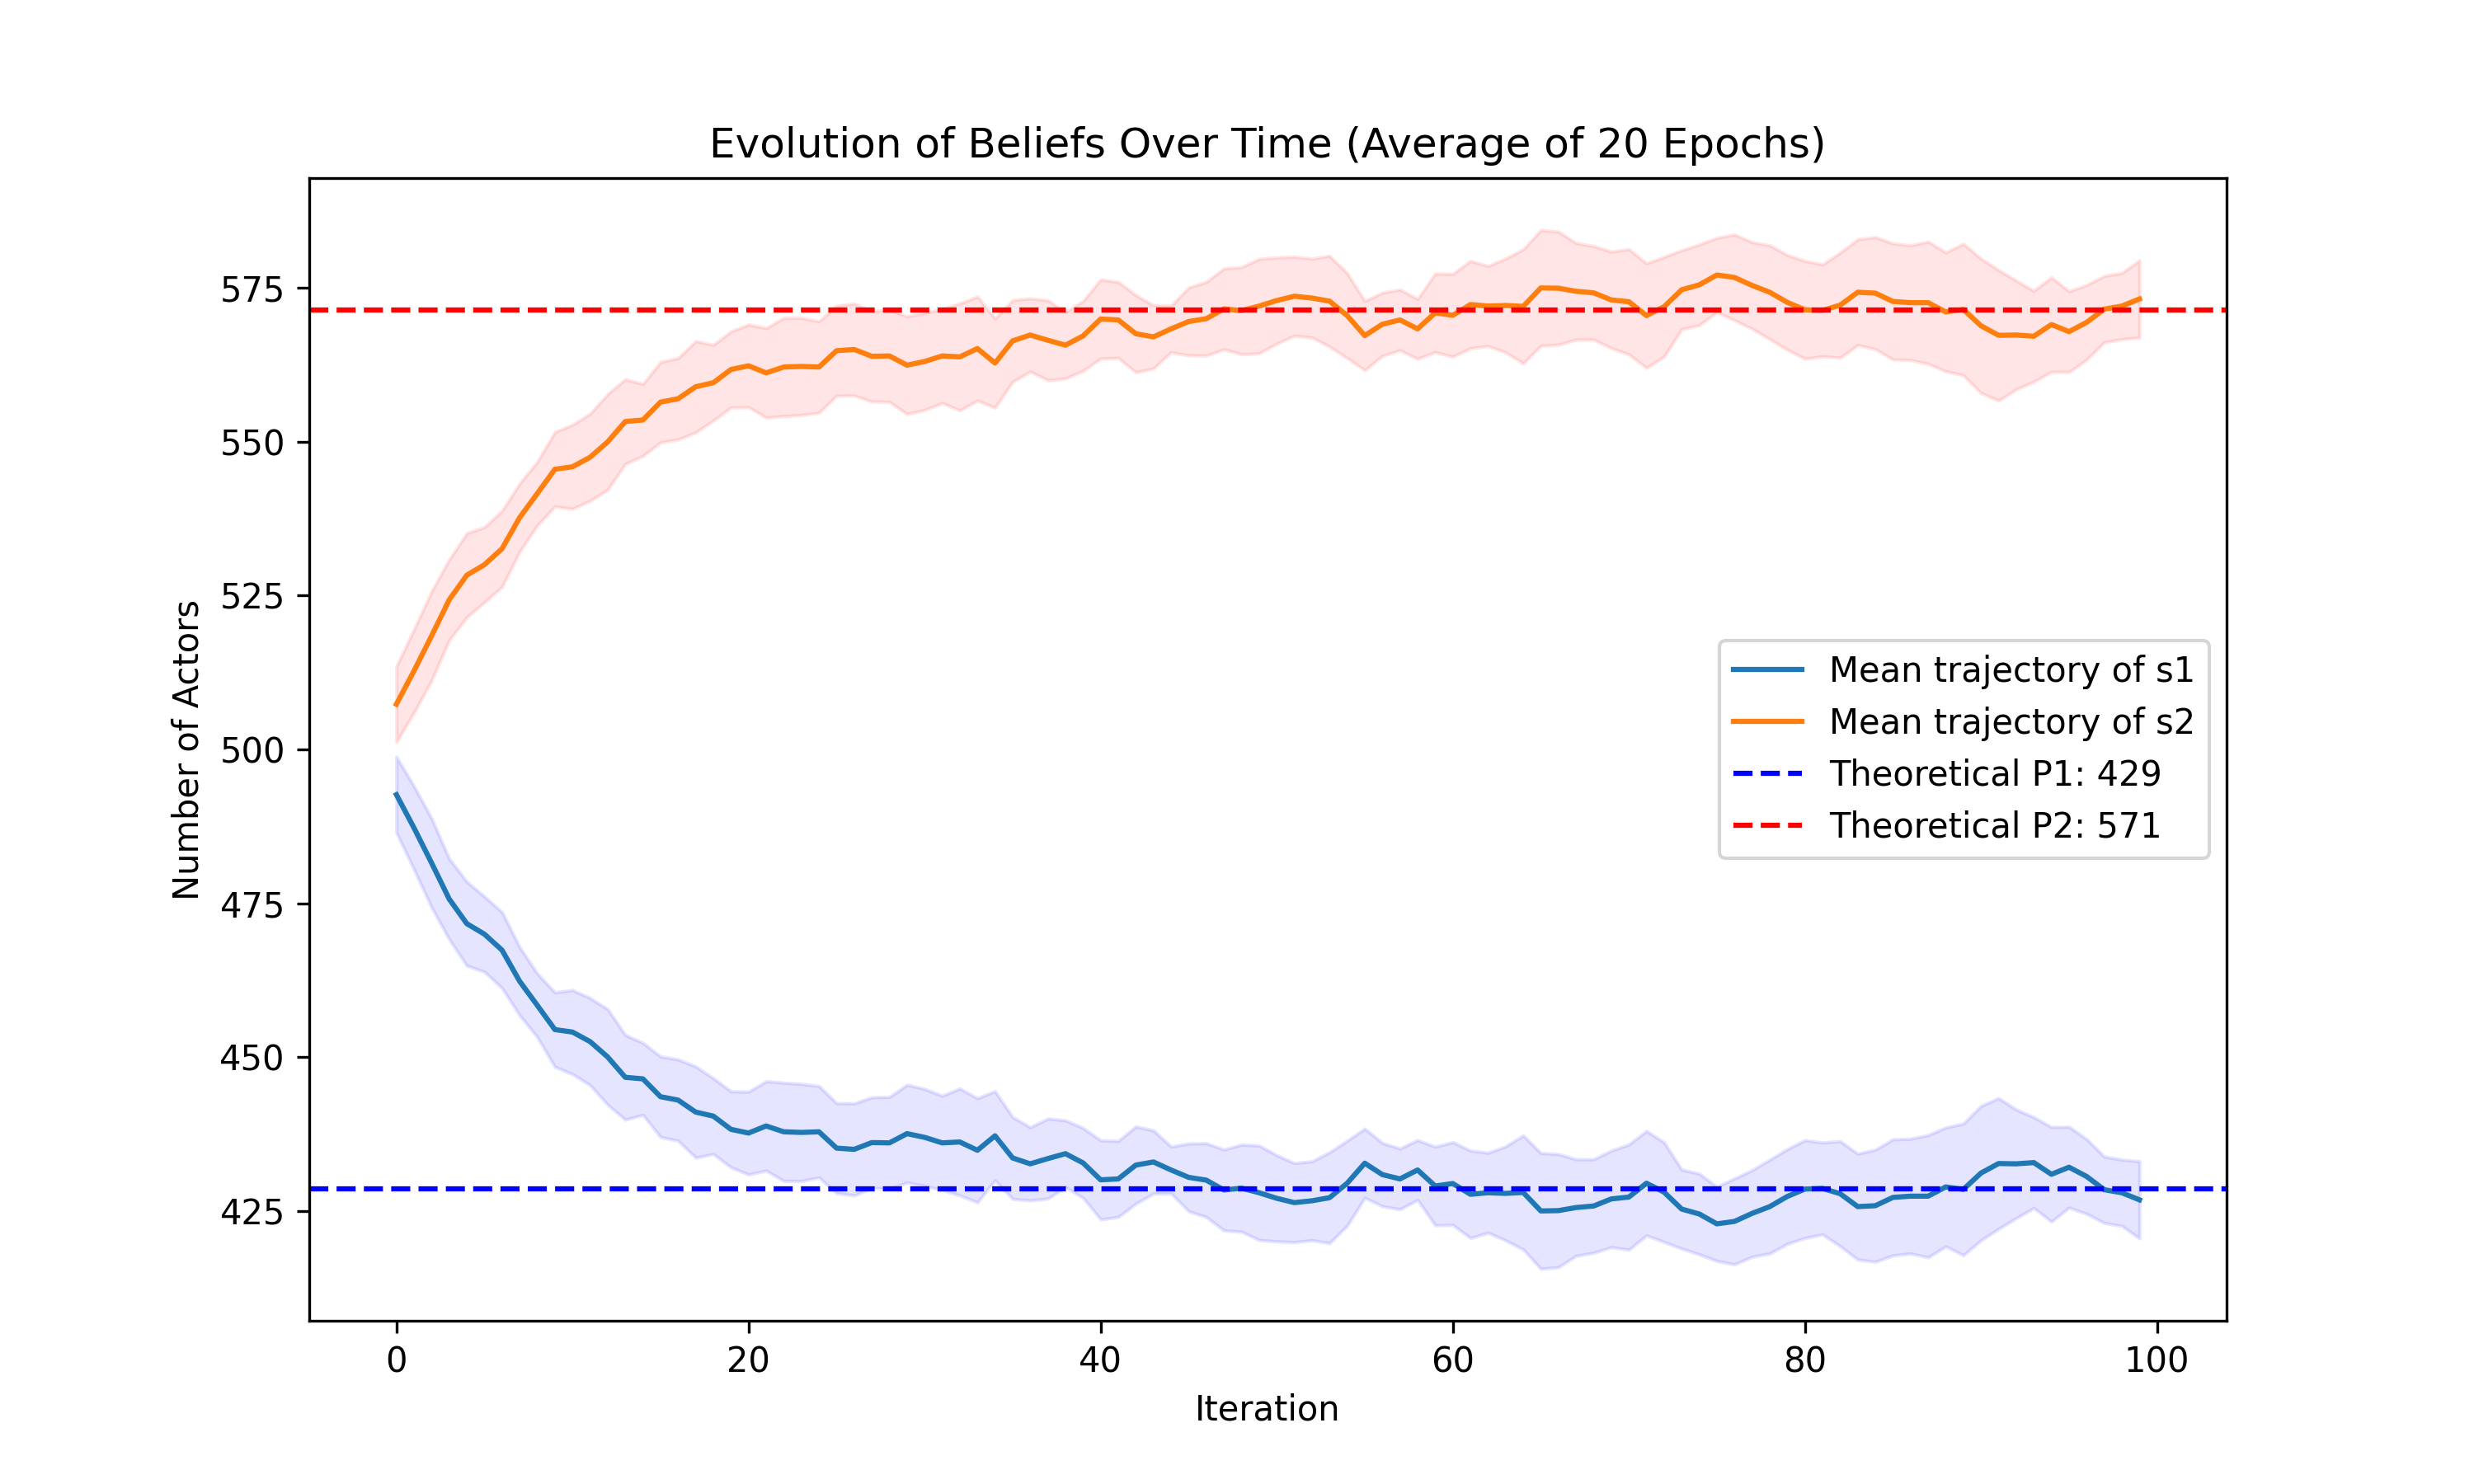
\includegraphics[width=0.8\textwidth]{FOO_Figure1.png}
    \caption{Evolution of beliefs over time, showcasing the dynamic changes in the network based on the specified interaction parameters.}
    \label{fig:evolution_of_beliefs_1}
\end{figure}

\begin{figure}[h]
    \centering
    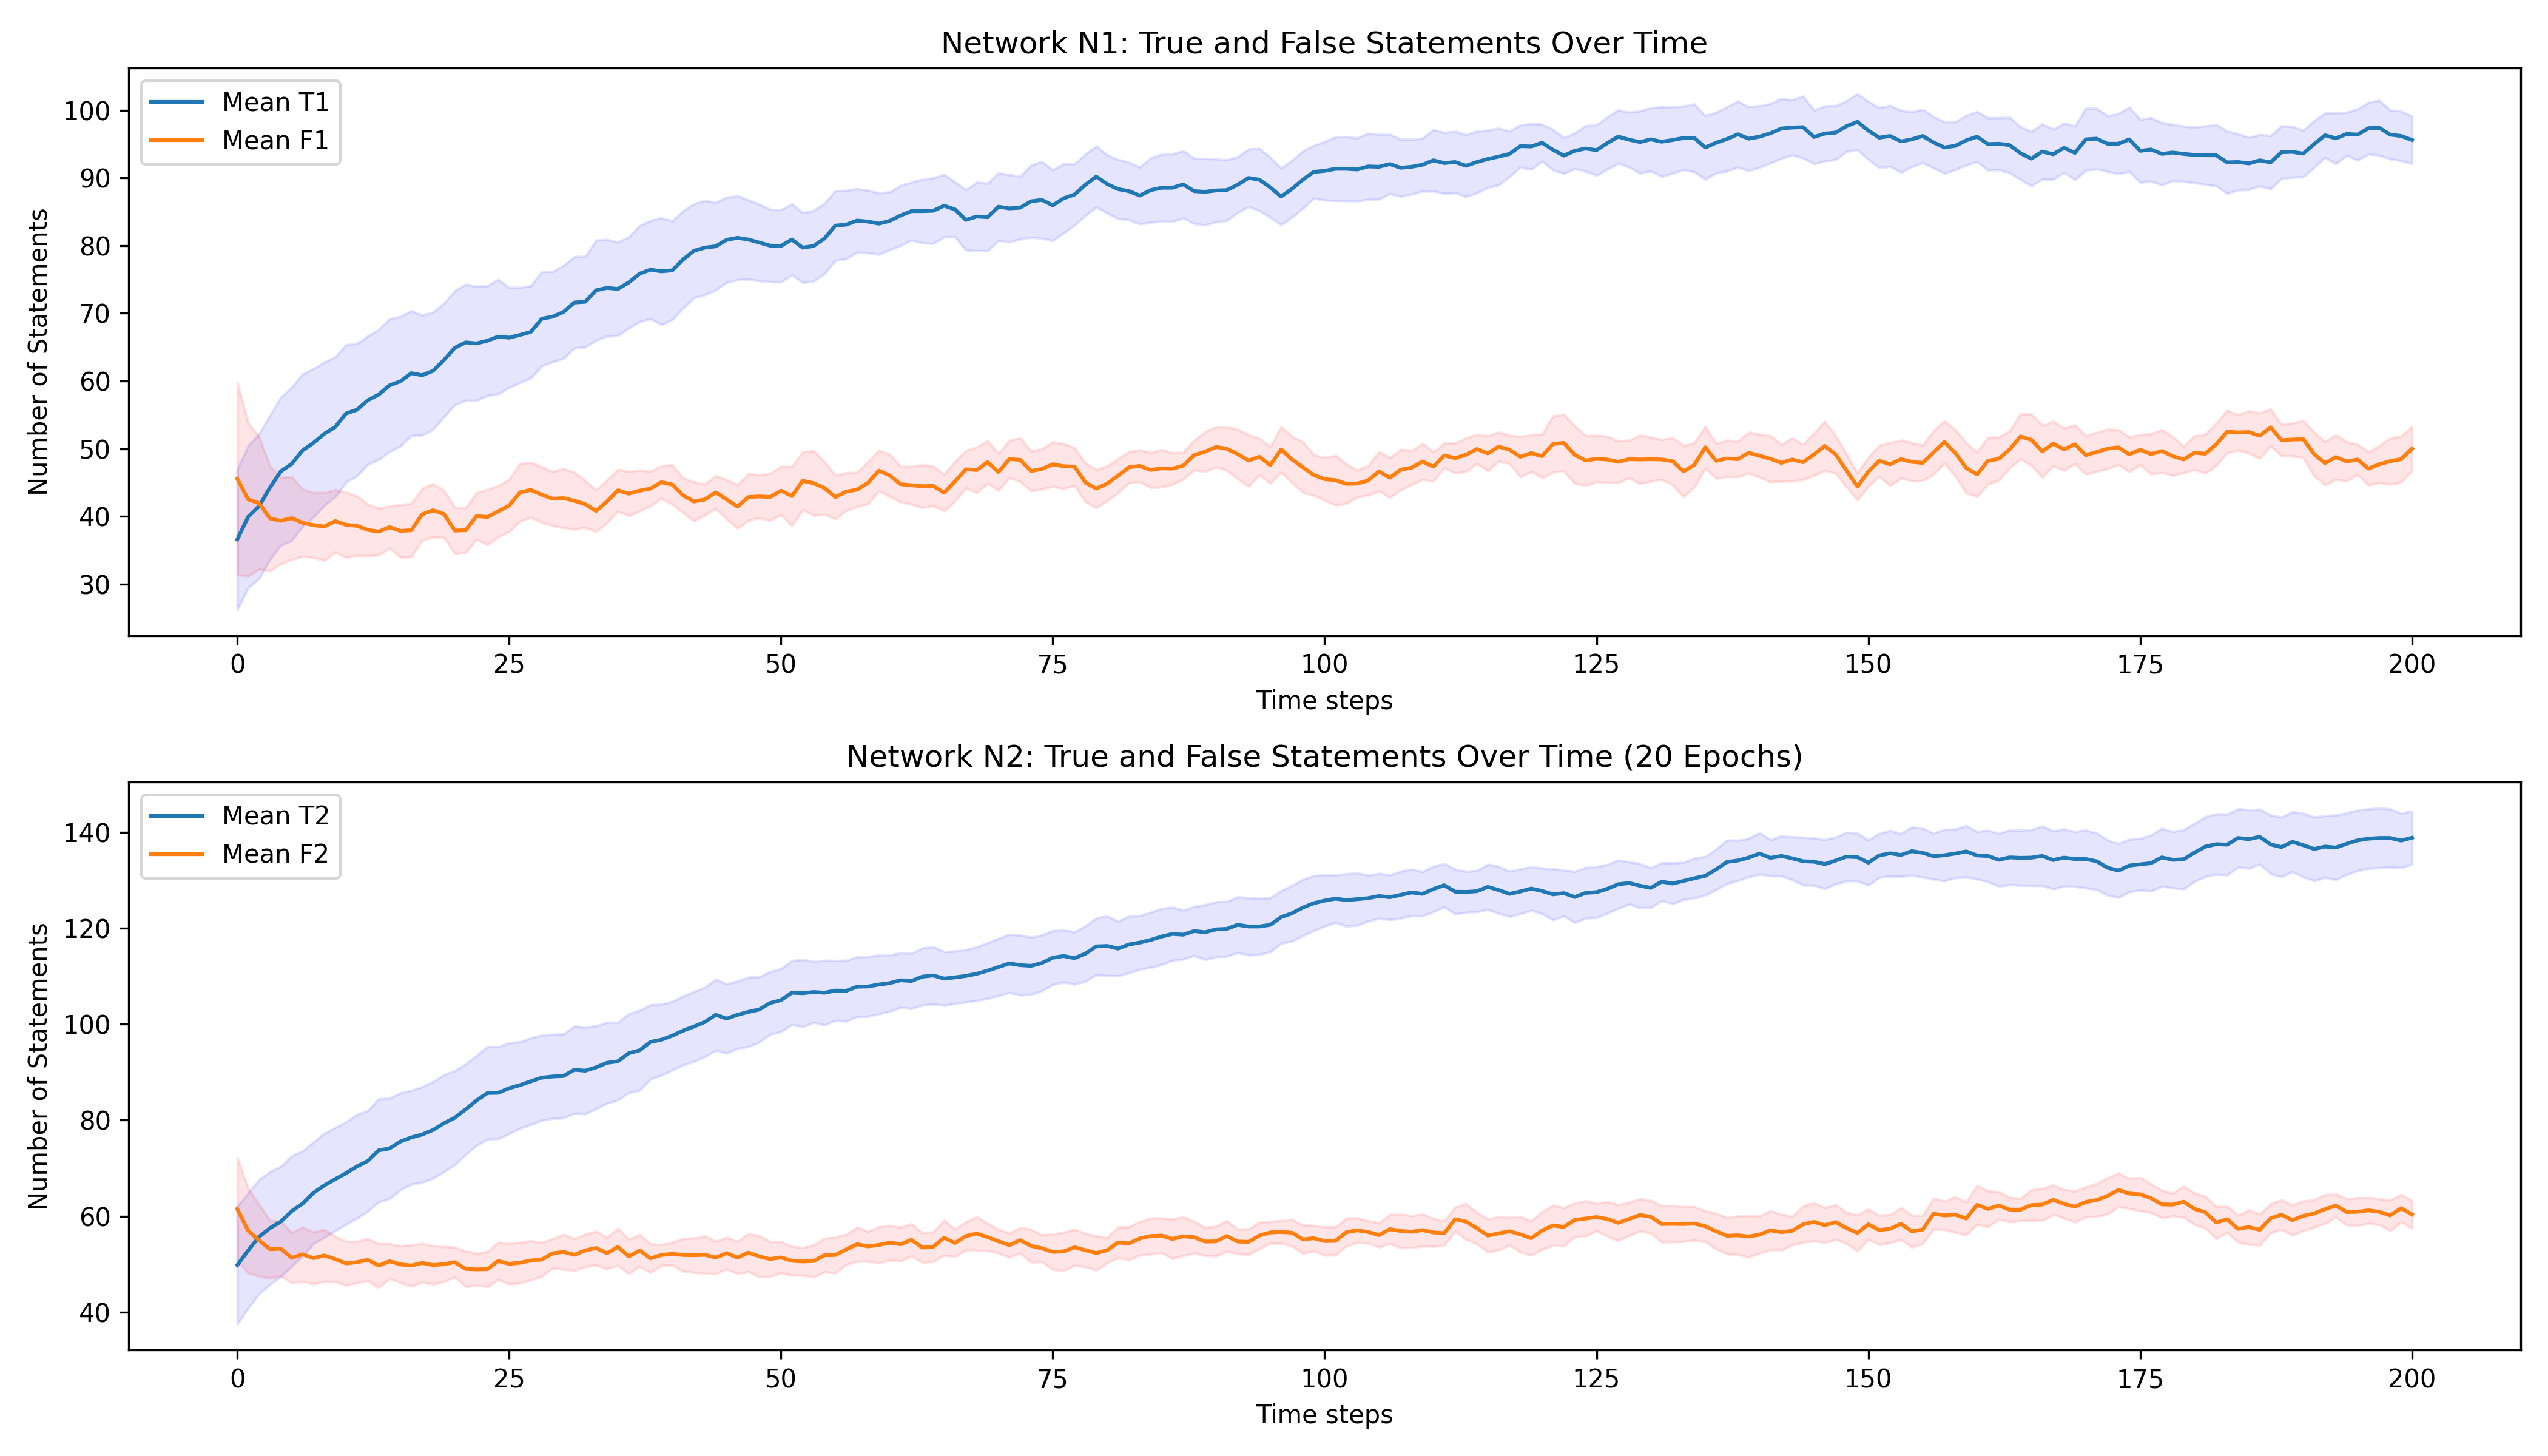
\includegraphics[width=0.8\textwidth]{FOO_Figure2.png}
    \caption{Evolution of beliefs over time, showcasing the dynamic changes in the network based on the specified interaction parameters.}
    \label{fig:evolution_of_beliefs_4}
\end{figure}


%===============================================
\subsection{Invalidation Consensus Algorithm}
%===============================================
The following sections detail a methodology for handling requests using multiple Large Language Models (LLMs) to ensure a high reliability and consistency in the responses generated by distributed systems. This approach is critical in scenarios where decision-making requires integration of diverse perspectives or knowledge bases, as often encountered in complex AI systems.

The process initiates with a request which acts as an input requiring processing. This request is then distributed among several instances of LLMs, labeled as LLM$_1$ to LLM$_n$. Each of these models processes the request independently and generates respective outputs, denoted as O$_1$ to O$_n$. Following the processing, all outputs are collected and assembled for a comparison.

A crucial step in this workflow is the assessment of whether the outputs differ significantly among the models. If significant differences are detected, indicating a lack of consensus, the system injects additional instructions aimed at consensus-building among the models. This might involve recalibration of model parameters or redefinition of input preprocessing. The request is then resent through the system until the outputs converge sufficiently, ensuring consistency. If no significant differences are found during the comparison, the system deems the results consistent enough to formulate a final response based on the collective outputs of the models, thus ending the process.

The algorithm presented in our study is closely aligned with the invalidation model designed to simulate and analyze the dynamics of belief changes within a discursive network, influenced by both true and false statements. This relationship is foundational for understanding the algorithm's purpose and its operational dynamics within the context of the proposed model. Below, we elaborate on how the algorithm relates to the invalidation model:

The invalidation model we introduced operates on a Markov chain framework that depicts the stochastic transitions between belief states in a network of actors. These states are significantly influenced by true statements (\(s_1\)) and false statements (\(s_2\)), wherein the interactions among actors can either reinforce or alter their current beliefs.


%===============================================
\subsubsection{Algorithm Steps and Their Functions}
%===============================================
\begin{enumerate}
    \item \textbf{Initialization and Distribution}: The process starts by initializing a request, symbolizing the input or stimulus that prompts interaction within the network. This request is distributed among various instances of large language models (LLMs), simulating the diverse responses of actors within the network.
    
    \item \textbf{Processing by LLMs}: Each LLM processes the request independently, mirroring the individual actor’s processing of information or statements within the network. This independence is crucial for capturing the varied interpretations and reactions among different actors based on their perspectives or biases.
    
    \item \textbf{Assembly and Difference Checking}: After processing, the outputs from all LLMs are assembled for comparison. This step is analogous to aggregating different beliefs or reactions within the network to assess consensus or discord.
    
    \item \textbf{Consensus and Response Generation}: If significant differences are detected, the algorithm injects consensus instructions and reiterates the process, reflecting the ongoing adjustments and interactions in the network as actors influence each other and gradually move towards a common understanding or belief. If no significant differences are detected, a response based on collective outputs is generated, signifying the stabilization of beliefs across the network.
\end{enumerate}

%===============================================
\subsubsection{Integration with Invalidation Dynamics}
%===============================================
The algorithm effectively integrates the dynamics of invalidation by considering how false information (represented by \(s_2\)) can influence the network's belief system and how true information (represented by \(s_1\)) can be reasserted. The use of LLMs to simulate this process provides a robust framework for exploring the complex interplay of information dissemination, belief formation, and change within large, interactive networks.


\begin{algorithm}
\caption{Consensus-based Response Generation using Multiple LLMs}
\begin{algorithmic}[1]
\Require Input request
\Ensure Consistent response from multiple LLMs

\State Initialize \(Request\)
\State Distribute \(Request\) to multiple LLMs \(LLM_1, LLM_2, \ldots, LLM_n\)

\For{\(i = 1\) to \(n\)}
    \State \(O_i \leftarrow LLM_i(Process(Request))\)
\EndFor

\State Assemble outputs \(O_1, O_2, \ldots, O_n\)
\State \(Difference \leftarrow CheckDifferences(O_1, O_2, \ldots, O_n)\)

\If{\(Difference = \text{True}\)}
    \State Add Consensus Instructions
    \State Go to Step 2
\Else
    \State \(Response \leftarrow GenerateResponse(O_1, O_2, \ldots, O_n)\)
    \State Output \(Response\)
\EndIf

\end{algorithmic}
\end{algorithm}

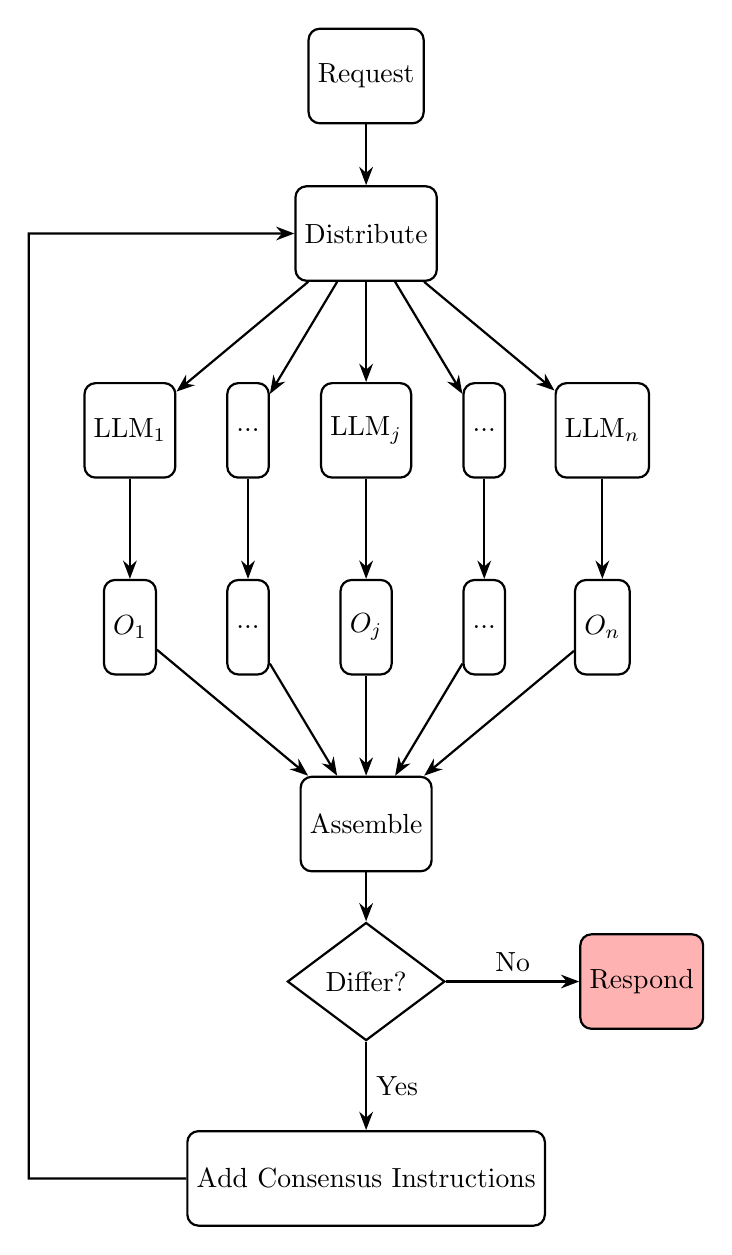
\begin{tikzpicture}[node distance=1.5cm and 2cm, >=Stealth, thick]

    % Define the styles
    \tikzstyle{block} = [rectangle, draw, text centered, rounded corners, minimum height=1.2cm]
    \tikzstyle{arrow} = [->, thick]
    \tikzstyle{circle} = [circle, fill, inner sep=1.5pt]
    \tikzstyle{decision} = [diamond, draw, text centered, minimum width=2cm, minimum height=1.5cm, inner sep=0pt]
    \tikzstyle{stop} = [rectangle, draw, text centered, rounded corners, minimum height=1.2cm, fill=red!30]

    % Nodes
    \node (request) [block] {Request};
    \node (cir) [block, below of=request, yshift=-0.5cm] {Distribute};

    \node (llm1) [block, below of=cir, xshift=-3cm, yshift=-1cm] {LLM$_1$};
    \node (dots1) [block, right of=llm1] {...};
    \node (llmj) [block, right of=dots1] {LLM$_j$};
    \node (dots2) [block, right of=llmj] {...};
    \node (llmn) [block, right of=dots2] {LLM$_n$};
    
    \node (o1) [block, below of=llm1, yshift=-1cm] {$O_1$};
    \node (dots3) [block, right of=o1] {...};
    \node (oj) [block, below of=llmj, yshift=-1cm] {$O_j$};
    \node (dots4) [block, right of=oj] {...};
    \node (on) [block, below of=llmn, yshift=-1cm] {$O_n$};
    
    \node (concat) [block, below of=dots3, xshift=1.5cm, yshift=-1cm] {Assemble};
    \node (decision) [decision, below of=concat, yshift=-0.5cm] {Differ?};
    \node (stop) [stop, right of=decision, xshift=2cm] {Respond};
    \node (consensus) [block, below of=decision, yshift=-1cm] {Add Consensus Instructions};
    
    % Arrows
    \draw [arrow] (request) -- (cir);
    \draw [arrow] (cir) -- (llm1);
    \draw [arrow] (cir) -- (dots1);
    \draw [arrow] (cir) -- (llmj);
    \draw [arrow] (cir) -- (dots2);
    \draw [arrow] (cir) -- (llmn);
    
    \draw [arrow] (llm1) -- (o1);
    \draw [arrow] (dots1) -- (dots3);
    \draw [arrow] (llmj) -- (oj);
    \draw [arrow] (dots2) -- (dots4);
    \draw [arrow] (llmn) -- (on);
    
    \draw [arrow] (o1) -- (concat);
    \draw [arrow] (oj) -- (concat);
    \draw [arrow] (on) -- (concat);
    \draw [arrow] (dots3) -- (concat);
    \draw [arrow] (dots4) -- (concat);
    
    \draw [arrow] (concat) -- (decision);
    \draw [arrow] (decision) -- node[anchor=west] {Yes} (consensus);
    
    % Curved arrow from consensus to decision
    \draw [arrow] (consensus.west) -- ++(-2,0) -- ++(0,12) -- (cir.west);
    \draw [arrow] (decision.east) -- node[anchor=south] {No} (stop.west);
    
\end{tikzpicture}

%===============================================
\section{Conclusion}
%===============================================

[TO DO: Clean up conclusions. Ensure that we cite the context int he intro, and address how this approach improves over the state of the  art.]

The numerical simulations serve as a powerful tool to understand and predict how beliefs propagate and evolve in a discursive network, illustrating the impact of interaction frequency and statement validity. The use of a Poisson distribution for modeling interaction counts adds a layer of realism and adaptability to the simulations, enhancing their applicability to real-world social dynamics.

To connect the refined model of belief propagation and verification energy to large language models (LLMs), we need to understand how LLMs generate statements and how they can be used to detect falsehoods. LLMs, such as GPT-4, generate text based on patterns they have learned from vast amounts of training data. These models do not have an inherent understanding of truth or falsehood but instead generate responses that are statistically likely given the input prompt and their training data. Here’s how this relates to our model: LLMs are trained on diverse datasets that include both true (type $s_1$) and false (type $s_2$) statements. When generating a response, the LLM samples from this learned distribution, which may include falsehoods if they appear frequently in the training data. In our model, verifying true statements ($s_1$) requires more energy. Similarly, generating true and accurate information often requires more context, deeper understanding, and reasoning, which the LLM might not always apply if not explicitly prompted to do so. Generating a plausible-sounding but false statement ($s_2$) might be "easier" in terms of the model's operations, similar to how $s_2$ statements deplete less energy. Unlike humans who can verify facts through external sources or reasoning, LLMs rely solely on their training data and prompt context. Without a mechanism to validate information against a ground truth, LLMs may produce statements that are statistically likely but false, akin to our model where falsehoods ($s_2$) require less verification energy and can propagate more easily.

Using multiple LLMs to spot falsehoods can be more effective than relying on a single model due to several factors that align with our refined model of belief propagation and verification energy. Multiple LLMs trained on different datasets or with different architectures can provide diverse perspectives. When multiple models analyze the same statement, they can cross-verify the information. If one model generates an $s_2$ statement, other models can provide additional context or challenge the falsehood based on their own learned patterns, similar to increasing the interaction frequency with true statements ($s_1$) in our model. Relying on a single LLM increases the risk of errors or biases inherent in that model’s training data. By consulting multiple models, we can reduce the likelihood of propagating falsehoods as different models may have different biases and strengths, leading to a more balanced and accurate output. In our model, verification energy depletes quickly when verifying true statements. Multiple LLMs can distribute this verification load. If verifying $s_1$ depletes energy, having multiple models can effectively pool their verification capacities, ensuring that the energy required to confirm the truth is distributed and managed better. This is analogous to having a collaborative verification process where the burden is shared. When multiple LLMs are used to evaluate a statement, we can derive a consensus based on the majority or weighted agreement. If most models agree that a statement is true or false, this consensus can act as a more reliable indicator than a single model’s output. This is similar to how higher interaction frequencies with true statements ($s_1$) in our model increase the likelihood of actors adopting $s_1$.

By connecting the refined model of belief propagation to the behavior of LLMs, we can better understand the generation and detection of false statements. LLMs generate false statements due to the probabilistic nature of their training data, analogous to how $s_2$ statements propagate more easily in a network with lower verification energy. Using multiple LLMs for falsehood detection is effective because it distributes the verification load, leverages diverse perspectives, and reduces individual biases, akin to increasing the interaction frequency with true statements and sharing verification energy in our model. This approach aligns with our understanding that collaborative verification and diverse interactions enhance the detection and correction of falsehoods in both human networks and AI systems.

Future research directions could include exploring additional techniques to mitigate invalidation, assessing the effectiveness of existing strategies in real-world applications, and examining the ethical implications of false information generated by LLMs. Addressing these challenges is essential for the responsible deployment and use of AI technologies.

The parallel between invalidation in LLMs and human discourse opens up new avenues for interdisciplinary research. It challenges us to consider invalidation not as a unique flaw of AI, but as a fundamental aspect of information processing that manifests across different types of cognitive systems. This perspective not only enriches our understanding of AI behavior but also provides a novel lens through which to examine human cognition and social dynamics.

The models presented for invalidaiton propagation provide a comprehensive framework for analyzing the dynamics of falsehood generation, propagation, and detection in isolated and interconnected discursive networks. It allows for the exploration of various scenarios by adjusting parameters such as falsehood generation rates, detection probabilities, and internal correction processes. Future work could focus on extending this model to include more complex network structures, heterogeneous actor behaviors, or the impact of targeted misinformation campaigns. Additionally, empirical studies could help validate the model's assumptions and refine its parameters for specific real-world contexts.

\bibliographystyle{plainnat}  
\bibliography{references}

\end{document}
